\documentclass[11pt]{article}

\usepackage[a4paper,margin=1in]{geometry}
\usepackage{amsmath,amssymb,mathtools}
\usepackage{siunitx}
\usepackage{graphicx}
\usepackage{booktabs}
\usepackage{tabularx}
\usepackage{threeparttable}
\usepackage{float}
\usepackage{xcolor}
\usepackage{hyperref}

\graphicspath{{./}{../}}

\hypersetup{
  colorlinks=true,
  linkcolor=blue,
  urlcolor=blue,
  citecolor=blue
}

\title{THz-TDS Time-Domain Fitting and Confidence-Map Studies}
\author{THzSim2 Lecture Package}
\date{\today}

\sisetup{
  group-separator={,},
  group-minimum-digits=4,
  per-mode=symbol
}

\newcommand{\eref}{E_{\mathrm{ref}}}
\newcommand{\esam}{E_{\mathrm{sam}}}
\newcommand{\efit}{E_{\mathrm{fit}}}
\newcommand{\eobs}{E_{\mathrm{obs}}}
\newcommand{\eps}{\varepsilon}
\newcommand{\epsinf}{\varepsilon_{\infty}}
\newcommand{\nt}{\tilde{n}}
\newcommand{\ii}{\mathrm{i}}
\newcommand{\dd}{\mathrm{d}}
\newcommand{\clight}{c_0}
\newcommand{\Jw}{\mathcal{J}_{w}}
\newcommand{\Erec}{\mathcal{E}_{\mathrm{rec}}}
\newcommand{\mstar}{m^\ast}
\newcolumntype{Y}{>{\raggedright\arraybackslash}X}

\begin{document}

\maketitle

\begin{abstract}
These notes describe THz-TDS time-domain fitting as a metrology problem rather than only a waveform-matching exercise. The final document combines forward-model theory, real measured fits, and recovery studies built from saved notebook outputs. In the present data set, measured transmission is the stronger real-data example, one-layer low-conductivity recovery is excellent in both transmission and reflection, high-conductivity one-layer transmission becomes globally non-unique, and oblique p-polarized high-conductivity reflection remains very strong. The advanced two-Drude epi study shows that transmission can recover selected channels well, whereas reflection under the present standard and parameterization is not yet quantitatively reliable. The emphasis throughout is on what the saved results justify conservatively for conductivity- and carrier-density-oriented wafer metrology.
\end{abstract}

\tableofcontents
\clearpage

\section{Why Time-Domain Fitting and Study Matter}

THz-TDS is not only a spectral intensity measurement. In a typical experiment the detector records the electric field as a function of time, so the data retain the phase of the field and the temporal ordering of physical events. The first transmitted or reflected pulse, later internal echoes, interference between partially overlapping pulses, and small shifts in arrival time are all part of the same measured trace. A time-domain fit uses this entire object directly. It asks whether a proposed optical stack, illuminated by the measured reference pulse, can reproduce the observed sample waveform.

Table~\ref{tab:notation-used-throughout} summarizes the notation used most often in the discussion. The same symbols are reused in the real-data fits and in the synthetic recovery studies so that the metrology interpretation stays connected to the underlying forward model.

\begin{table}[htbp]
\centering
\caption{Notation used throughout the lecture notes.}
\label{tab:notation-used-throughout}
\small
\begin{tabularx}{\linewidth}{@{}lY@{}}
\toprule
Symbol & Meaning \\
\midrule
\(\eref(t)\) & processed reference waveform in the time domain \\
\(\esam(t)\) & processed sample waveform in the time domain \\
\(H(\omega)\) & modeled transfer function that converts the measured reference into the predicted sample waveform \\
\(T(\omega)\) & transmission response of the modeled stack or selected transmission channel \\
\(R(\omega)\) & reflection response of the modeled stack or selected reflection channel \\
\(\sigma\) & conductivity, used as the main metrology quantity in the study discussion \\
\(\tau\) & carrier relaxation time, with \(\tau=\gamma^{-1}\) in the Drude parameterization \\
\(N\) & derived carrier density obtained from \(\sigma\) and \(\tau\) after choosing an effective mass \\
\(\omega_p\) & plasma frequency, which sets the free-carrier spectral weight \\
\(\gamma\) & scattering rate or damping rate in the Drude model \\
\bottomrule
\end{tabularx}
\end{table}

This is a stronger inverse problem than a reduced spectral workflow. A spectral workflow may first divide two Fourier spectra, unwrap the phase, infer an effective refractive index, isolate one echo delay, or fit a smooth conductivity spectrum. Such reductions can be useful, but they usually discard part of the measurement context or require intermediate choices that are not themselves physical parameters of the sample. A time-domain fit instead keeps the measured pulse as the source term and compares the predicted and observed waveforms after all modeled propagation, interface reflection, absorption, dispersion, and reference-standard effects have acted together. The fit is therefore constrained not only by spectral magnitude, but also by phase, timing, echo structure, and the causal sequence of the waveform.

It is important to separate two questions that are often conflated. Fitting a waveform once means finding the parameter vector that gives the best agreement for one measured trace. This is the usual inverse problem for one sample under one set of preprocessing choices and one assumed forward model. A study asks a broader metrology question. It chooses truth parameters, simulates measurements from those truths, adds controlled noise, refits the synthetic traces, and compares the recovered parameters with the values that generated the data. A study therefore probes whether the fitting procedure can recover the right physical quantities, not merely whether it can make a visually plausible waveform.

The confidence maps used in these notes are maps of recoverability over a chosen parameter plane. Each map point represents a synthetic truth case and a refit. Low recovery error means that the inverse procedure returns the correct physical parameters under the chosen geometry, model, bounds, noise level, and reference standard. High recovery error means that the measurement and model do not determine those parameters reliably in that region, even if the fitted waveform may still look acceptable. In this sense a confidence map is closer to an operational envelope for metrology than to a plot of detector sensitivity.

\section{Why Time-Domain Fit is Often Better}

The main advantage of time-domain fitting is that it respects the causal structure of the measurement. A THz pulse interacts with each interface and layer in a definite temporal order. Some parts of the waveform are dominated by the directly transmitted or reflected pulse, while later parts carry internal round trips, substrate echoes, or weak reflections from buried interfaces. When the fit is performed in the time domain, these delayed events remain visible as separate constraints whenever the bandwidth and time window allow them to be resolved. Even when echoes overlap, their interference still changes the shape and phase of the waveform in a way that a forward model can exploit.

Time-domain fitting also uses the measured reference pulse in a natural way. The reference trace contains the actual source spectrum, detector response, finite bandwidth, phase chirp, and any reproducible instrument filtering that survive preprocessing. In the forward calculation, the model does not need to invent an ideal incident pulse. It multiplies the Fourier transform of the measured reference by the sample transfer function and then transforms back to time. This makes the simulation a model of how the measured instrument pulse would appear after passing through, or reflecting from, the proposed optical stack.

Another practical strength is robustness against fragile phase-extraction steps. In a purely spectral inversion, the sample-to-reference ratio must be interpreted as a complex transfer function over a finite and noisy band. Phase unwrapping, windowing, zeros in the reference spectrum, and weak high-frequency signal can all introduce artifacts before the physical model is fitted. A time-domain objective does not remove these issues, but it postpones the comparison until after the forward model has predicted the measured waveform. The fit can therefore use timing and waveform shape directly, rather than requiring a separately stabilized refractive-index or conductivity spectrum as an intermediate product.

The same framework can treat transmission, reflection, oblique incidence, polarization, and reference standards without changing the basic inverse-problem structure. The electromagnetic model produces a transmission response \(T(\omega)\) or a reflection response \(R(\omega)\), and the observable transfer function \(H(\omega)\) is formed relative to the relevant measurement standard. This is especially important in reflection, where the measured trace is usually meaningful only relative to a mirror, a bare substrate, or another reference stack. Time-domain fitting makes this standard part of the physical model rather than an afterthought.

These advantages do not make the inverse problem automatically unique. Different parameter combinations can produce nearly indistinguishable waveforms over the measured bandwidth, especially when thickness, conductivity, scattering time, delay, scale, and reference mismatch trade off against one another. A small residual is therefore not proof that the fitted parameters are the only possible physical explanation. Preprocessing can also move the answer: baseline removal, pulse alignment, time-window selection, apodization, and treatment of weak echoes all change which parts of the waveform carry the most weight. Model incompleteness is another serious limitation. Surface roughness, anisotropy, inhomogeneous carrier profiles, non-Drude response, imperfect standards, beam effects, and sample misalignment can all be absorbed into apparently reasonable fitted parameters if the model does not represent them explicitly. Finally, because the fit is always made to a normalized measurement, assumptions about the reference pulse and the reference standard remain part of the inferred physics. Time-domain fitting is powerful precisely because it uses more of the measurement, but that also means its conclusions inherit more of the measurement chain.

\section{Forward Model Theory}

Let \(\eref(t)\) denote the processed reference waveform and let its Fourier transform be
\begin{equation}
  \hat{\eref}(\omega)
  =
  \int_{-\infty}^{\infty}\eref(t)\exp(-\ii\omega t)\,\dd t .
  \label{eq:reference_transform}
\end{equation}
The predicted sample waveform is built in the frequency domain as
\begin{equation}
  \hat{\esam}(\omega)
  =
  H(\omega)\hat{\eref}(\omega),
  \label{eq:sample_spectrum}
\end{equation}
followed by an inverse Fourier transform. The central object is the complex transfer function \(H(\omega)\). It is not a material property by itself. It is the electromagnetic response of the modeled measurement: the selected transmission or reflection channel of the optical stack, usually divided by the corresponding response of a reference standard. Thus \(H(\omega)\) may represent a transmitted sample relative to a blank aperture, a reflected sample relative to a mirror, or an epi-coated wafer relative to a bare-substrate standard. The mathematical role is always the same: \(H(\omega)\) tells the measured reference pulse how to become the predicted sample pulse.

The stack model begins by assigning each layer \(j\) a thickness \(d_j\) and a complex permittivity \(\eps_j(\omega)\). The corresponding complex refractive index is
\begin{equation}
  \nt_j(\omega)=\sqrt{\eps_j(\omega)} .
  \label{eq:complex_index}
\end{equation}
The branch is chosen so that passive media attenuate rather than amplify the field. With the time convention used in Eq.~\eqref{eq:reference_transform}, this corresponds to selecting the branch for which the forward propagating field has non-negative absorption.

At oblique incidence, the transverse component of the wave vector is conserved across all planar interfaces. If the incident medium is labeled \(0\) and the external incidence angle is \(\theta_0\), then the invariant transverse index is \(\nt_0\sin\theta_0\). The longitudinal direction in layer \(j\) is represented by
\begin{equation}
  \cos\theta_j
  =
  \sqrt{
    1-
    \left(
      \frac{\nt_0\sin\theta_0}{\nt_j}
    \right)^2
  },
  \label{eq:complex_cosine}
\end{equation}
again with the branch chosen for forward propagation or forward attenuation. The propagation factor through the layer is then
\begin{equation}
  P_j(\omega)
  =
  \exp\!\left(
    \ii\omega \nt_j(\omega)\cos\theta_j
    \frac{d_j}{\clight}
  \right).
  \label{eq:propagation_factor}
\end{equation}
This phase factor is where the thickness, optical delay, dispersion, and absorption of a layer enter the transfer function.

The next ingredient is the interface response. For an interface from medium \(j\) to medium \(k\), the Fresnel coefficients for \(s\) polarization are
\begin{align}
  r_{jk}^{s}
  &=
  \frac{\nt_j\cos\theta_j-\nt_k\cos\theta_k}
       {\nt_j\cos\theta_j+\nt_k\cos\theta_k},
  &
  t_{jk}^{s}
  &=
  \frac{2\nt_j\cos\theta_j}
       {\nt_j\cos\theta_j+\nt_k\cos\theta_k}.
  \label{eq:fresnel_s}
\end{align}
For \(p\) polarization the coefficients are
\begin{align}
  r_{jk}^{p}
  &=
  \frac{\nt_k\cos\theta_j-\nt_j\cos\theta_k}
       {\nt_k\cos\theta_j+\nt_j\cos\theta_k},
  &
  t_{jk}^{p}
  &=
  \frac{2\nt_j\cos\theta_j}
       {\nt_k\cos\theta_j+\nt_j\cos\theta_k}.
  \label{eq:fresnel_p}
\end{align}
The Fresnel coefficients determine how much field is reflected or transmitted at each boundary, while \(P_j\) determines the phase and attenuation accumulated between boundaries. Multiple internal reflections are generated by repeated combinations of these same factors.

For a single finite layer \(1\) between an incident medium \(0\) and an exit medium \(2\), the finite Fabry--Perot transmission response with at most \(M\) internal round trips can be written
\begin{equation}
  T_M(\omega)
  =
  t_{01}(\omega)P_1(\omega)t_{12}(\omega)
  \sum_{m=0}^{M}
  z^m(\omega),
  \qquad
  z(\omega)=r_{10}(\omega)P_1(\omega)r_{12}(\omega)P_1(\omega).
  \label{eq:finite_single_layer_transmission}
\end{equation}
The corresponding reflection response is
\begin{equation}
  R_M(\omega)
  =
  r_{01}(\omega)
  +
  t_{01}(\omega)P_1(\omega)r_{12}(\omega)P_1(\omega)t_{10}(\omega)
  \sum_{m=0}^{M-1}z^m(\omega).
  \label{eq:finite_single_layer_reflection}
\end{equation}
Equations~\eqref{eq:finite_single_layer_transmission} and \eqref{eq:finite_single_layer_reflection} make the physical interpretation transparent. The first transmitted term enters the slab, propagates across it, and exits. Each additional term adds one more internal round trip. In reflection, the first term is the prompt front-surface reflection, while the second group contains fields that enter the slab, reflect from the back interface, and return through the front.

For a general isotropic multilayer stack, the same physics is assembled recursively. Suppose \(R_{j+1}(\omega)\) and \(T_{j+1}(\omega)\) are the effective reflection and transmission responses of everything behind layer \(j\), as seen after the interface into the following medium. The denominator
\begin{equation}
  D_j(\omega)
  =
  1-
  r_{j+1,j}(\omega)P_j(\omega)
  R_{j+1}(\omega)P_j(\omega)
  \label{eq:recursive_denominator}
\end{equation}
sums the infinite sequence of round trips between the front side of layer \(j\) and the effective reflector behind it. The effective transmission and reflection looking into that part of the stack are then
\begin{align}
  T_j(\omega)
  &=
  \frac{
    t_{j,j+1}(\omega)P_j(\omega)T_{j+1}(\omega)
  }{
    D_j(\omega)
  },
  \label{eq:recursive_transmission}
  \\
  R_j(\omega)
  &=
  r_{j,j+1}(\omega)
  +
  \frac{
    t_{j,j+1}(\omega)P_j(\omega)
    R_{j+1}(\omega)P_j(\omega)t_{j+1,j}(\omega)
  }{
    D_j(\omega)
  }.
  \label{eq:recursive_reflection}
\end{align}
Starting from the last interface and applying this recursion back toward the incident medium gives the full stack response. This is the numerical generalization of the elementary Fabry--Perot series: interfaces supply Fresnel amplitudes, layers supply propagation phases, and the recursion sums the multiply reflected paths.

The raw stack channel is not always the final measured transfer function. If \(Q_{\mathrm{sample}}(\omega)\) denotes the selected sample channel, either \(T_{\mathrm{sample}}(\omega)\) or \(R_{\mathrm{sample}}(\omega)\), and \(Q_{\mathrm{std}}(\omega)\) denotes the corresponding response of the measurement standard, then the modeled observable is
\begin{equation}
  H(\omega)
  =
  \frac{Q_{\mathrm{sample}}(\omega)}
       {Q_{\mathrm{std}}(\omega)} .
  \label{eq:standard_normalization}
\end{equation}
When the standard is unity this reduces to the raw stack channel. Otherwise the standard removes the response of the chosen reference measurement and defines what the fitted waveform means experimentally. The predicted sample trace is finally obtained by inserting \(H(\omega)\) into Eq.~\eqref{eq:sample_spectrum} and transforming back to time.

\subsection{Single-Layer Example and Recovery of the Airy Formula}

The simplest useful example is a plane wave at normal incidence on a single slab of thickness \(d\) and constant complex refractive index
\begin{equation}
  \nt = n+\ii\kappa .
  \label{eq:constant_complex_index}
\end{equation}
The slab is surrounded by two semi-infinite media with refractive indices \(n_0\) and \(n_2\). At normal incidence there is no distinction between \(s\) and \(p\) polarization for the scalar Fresnel amplitudes, so
\begin{equation}
  r_{jk}=\frac{n_j-n_k}{n_j+n_k},
  \qquad
  t_{jk}=\frac{2n_j}{n_j+n_k},
  \label{eq:normal_fresnel}
\end{equation}
where \(n_1=\nt\). The one-way propagation factor through the slab is
\begin{equation}
  P(\omega)=\exp\!\left(\ii\omega\nt\frac{d}{\clight}\right).
  \label{eq:single_layer_propagation}
\end{equation}

The directly transmitted field amplitude is \(t_{01}Pt_{12}\). A contribution that makes one additional round trip inside the slab acquires the factor \(r_{12}Pr_{10}P\). Two additional round trips acquire the square of this factor, and so on. The full transmitted amplitude is therefore the Fabry--Perot series
\begin{equation}
  T(\omega)
  =
  t_{01}Pt_{12}
  \left[
    1+
    r_{12}Pr_{10}P+
    \left(r_{12}Pr_{10}P\right)^2+
    \cdots
  \right].
  \label{eq:fp_transmission_series}
\end{equation}
For a passive slab the round-trip magnitude is less than unity over the physical band, and the geometric series gives
\begin{equation}
  T(\omega)
  =
  \frac{
    t_{01}t_{12}P
  }{
    1-r_{12}r_{10}P^2
  } .
  \label{eq:airy_transmission}
\end{equation}
This is the standard Airy-type transmission form written in field amplitudes.

The reflection amplitude has a prompt front-interface term and a sequence of internally reflected terms. The first internal contribution enters the slab, propagates to the back interface, reflects, propagates back, and exits into the incident medium:
\begin{equation}
  t_{01}Pr_{12}Pt_{10}.
  \label{eq:first_internal_reflection}
\end{equation}
Every later internal contribution is multiplied by the same round-trip factor \(r_{12}Pr_{10}P\). Thus
\begin{equation}
  R(\omega)
  =
  r_{01}
  +
  t_{01}Pr_{12}Pt_{10}
  \left[
    1+
    r_{12}Pr_{10}P+
    \left(r_{12}Pr_{10}P\right)^2+
    \cdots
  \right],
  \label{eq:fp_reflection_series}
\end{equation}
and summation gives
\begin{equation}
  R(\omega)
  =
  r_{01}
  +
  \frac{
    t_{01}t_{10}r_{12}P^2
  }{
    1-r_{12}r_{10}P^2
  } .
  \label{eq:airy_reflection}
\end{equation}
These formulas are the conceptual prototype of the multilayer calculation. The general code does not need a separate closed form for every possible stack, because the recursive forward model constructs the same physical object by combining Fresnel amplitudes, propagation factors, and multiple-reflection sums layer by layer.

\subsection{Drude and Two-Drude Material Models}

Many THz-TDS measurements of semiconductors, conductive films, doped layers, and photoexcited media are dominated by mobile charge carriers. The Drude model is the simplest causal free-carrier model that connects the optical response to carrier inertia and momentum relaxation. For one carrier population it writes the complex permittivity as
\begin{equation}
  \eps(\omega)
  =
  \epsinf
  -
  \frac{\omega_p^2}{\omega(\omega+\ii\gamma)} ,
  \label{eq:drude_permittivity}
\end{equation}
where \(\epsinf\) is the high-frequency background permittivity, \(\omega_p\) is the plasma frequency, and \(\gamma\) is the momentum-scattering rate. The relaxation time is
\begin{equation}
  \tau=\gamma^{-1}.
  \label{eq:tau_gamma}
\end{equation}
For carriers of density \(N\), charge magnitude \(e\), and effective mass \(m^\ast\), the plasma frequency satisfies
\begin{equation}
  \omega_p^2=\frac{Ne^2}{\varepsilon_0 m^\ast}.
  \label{eq:plasma_frequency}
\end{equation}
The DC conductivity is
\begin{equation}
  \sigma_0
  =
  \varepsilon_0\frac{\omega_p^2}{\gamma}
  =
  Ne\mu ,
  \qquad
  \mu=\frac{e\tau}{m^\ast},
  \label{eq:dc_conductivity_mobility}
\end{equation}
where \(\mu\) is the carrier mobility. Thus \(\omega_p\) primarily measures carrier spectral weight, while \(\gamma\) or \(\tau\) measures how quickly carrier momentum relaxes.

The same model can be written in terms of the complex conductivity,
\begin{equation}
  \sigma(\omega)
  =
  \frac{\sigma_0}{1-\ii\omega\tau},
  \qquad
  \eps(\omega)
  =
  \epsinf+\frac{\ii\sigma(\omega)}{\varepsilon_0\omega},
  \label{eq:drude_conductivity}
\end{equation}
with the sign convention matched to Eq.~\eqref{eq:reference_transform}. This form is often intuitive in the THz range. THz angular frequencies can be comparable to common carrier scattering rates in semiconductors and conducting oxides, so the measured band is sensitive not only to the amount of mobile charge but also to the finite time over which carrier velocity persists. In the low-frequency limit \(\omega\tau\ll 1\), the response approaches the DC conductivity. When \(\omega\tau\) is of order unity, the real and imaginary parts of \(\sigma(\omega)\) change strongly across the measured band, giving THz-TDS direct leverage on relaxation time and mobility.

A single Drude term assumes one effective carrier population with one scattering rate. Real layered or doped systems may not be so simple. Two spatial regions can conduct in parallel, such as a surface accumulation layer and a bulk channel. A film may contain carriers with different mobilities, or a photoexcited semiconductor may have electron and hole contributions with different effective masses and scattering times. In these cases a two-Drude model is a compact phenomenological extension:
\begin{equation}
  \eps(\omega)
  =
  \epsinf
  -
  \frac{\omega_{p1}^2}{\omega(\omega+\ii\gamma_1)}
  -
  \frac{\omega_{p2}^2}{\omega(\omega+\ii\gamma_2)} .
  \label{eq:two_drude_permittivity}
\end{equation}
Equivalently, the total conductivity is the sum of two Drude conductivities,
\begin{equation}
  \sigma(\omega)
  =
  \frac{\sigma_{01}}{1-\ii\omega\tau_1}
  +
  \frac{\sigma_{02}}{1-\ii\omega\tau_2}.
  \label{eq:two_drude_conductivity}
\end{equation}
The two terms should not be interpreted automatically as uniquely identified microscopic populations. They are physically motivated degrees of freedom that allow the model to represent two characteristic carrier time scales or two conduction channels. Because the additional freedom can introduce strong parameter correlations, a two-Drude fit is meaningful only when the measurement geometry, bandwidth, signal-to-noise ratio, and reference strategy provide enough information to separate the channels.

\section{How the Time-Domain Fit Works}

The time-domain fit is an iterative forward--inverse procedure. It begins with processed reference and sample traces on a common time grid. Preprocessing normally removes baseline offsets, chooses the time window to be fitted, aligns the reference and sample pulses to a consistent convention, and may suppress regions that are known to contain unrelated artifacts. These operations are not merely cosmetic. They define the data vector that the inverse problem will attempt to explain, and they determine which pulse features enter the objective most strongly.

The physical model is then expressed as a parameterized optical stack. Some quantities, such as a substrate permittivity or known layer thickness, may be fixed. Others are declared as fit variables with lower and upper bounds chosen from physically meaningful ranges. For a Drude layer, for example, the fitted variables may be a thickness, a relaxation time, and a conductivity, while the forward model internally converts those variables into \(\eps(\omega)\), \(\nt(\omega)\), Fresnel coefficients, and propagation factors. Bounds are important because unconstrained optical fits can otherwise move into parameter regions that produce a mathematically low residual but no plausible sample.

At each optimizer step the current parameter vector defines a complete stack. The forward solver constructs \(T(\omega)\) or \(R(\omega)\), applies the appropriate standard normalization to obtain \(H(\omega)\), multiplies the measured reference spectrum by \(H(\omega)\), and transforms the result back to the time domain. The calculated waveform \(\efit(t_k)\) is compared with the observed sample waveform \(\eobs(t_k)\) through a scalar objective. A typical weighted waveform objective is
\begin{equation}
  \Jw
  =
  \frac{
    \sum_k w_k\left[\efit(t_k)-\eobs(t_k)\right]^2
  }{
    \sum_k w_k\eobs^2(t_k)
  } .
  \label{eq:weighted_objective}
\end{equation}
The denominator makes the objective dimensionless and reduces trivial dependence on signal amplitude. The weights \(w_k\) are often constructed from a smoothed envelope of the observed trace. This emphasizes the main pulse and informative echoes, where the waveform contains phase and amplitude information about the stack, while preventing long low-amplitude tails or baseline regions from dominating simply because they contain many time samples.

The optimizer changes the fitted parameters until the objective is minimized within the specified bounds and convergence tolerances. In practical THz-TDS, the fit may also include nuisance parameters such as an amplitude scale, a small vertical offset, or a residual delay. A delay parameter is especially important when the preprocessing alignment is not exact or when the physical model and the measured reference define slightly different time origins. The delay is not a substitute for layer thickness, but it can prevent a small global timing error from being incorrectly absorbed into material parameters.

After convergence, the best-fit parameters describe the local optimum found by the optimizer. The residual waveform shows where the model still fails in time, while the corresponding spectral comparison can reveal bandwidth regions with systematic phase or amplitude disagreement. Near the optimum, the local sensitivity of the waveform to the fitted parameters can be approximated by a Jacobian matrix. From this Jacobian, together with the residual scale and objective weighting, one can estimate a local covariance matrix and the associated parameter-correlation matrix. This local uncertainty estimate is useful, but it is a statement about small parameter perturbations around one fitted solution. It does not by itself prove that the same solution would be recovered from other truth points, other noise realizations, or a different preprocessing choice.

\section{Correlation Matrix vs Study Confidence Map}

A fit-correlation matrix and a confidence map answer different uncertainty questions. The correlation matrix is local to one fit. It is computed from the sensitivity of the residual to small changes in the fitted variables near one optimum, usually through a Jacobian or approximate Hessian. If two parameters have a correlation coefficient close to \(+1\) or \(-1\), then the waveform can be changed very little by moving those parameters together in the indicated direction near that optimum. The matrix therefore diagnoses local trade-offs inside one solution.

This local view is necessary but incomplete. A nonlinear inverse problem can have broad valleys, disconnected minima, boundary attractions, or regions where the optimizer returns a plausible but wrong parameter set. These effects may not be visible from the covariance matrix at one nominal fit. A confidence map addresses a more global question by repeating the full inversion over a chosen plane of truth parameters. Instead of asking how parameters co-vary near one optimum, it asks where in the parameter plane the entire measurement-and-fitting procedure returns the correct values after noise is added.

The distinction matters for interpretation. A fit can have moderate local correlations and still fail globally if different truth points produce nearly indistinguishable waveforms. Conversely, a fit can show strong local correlation between two variables while the recovery of a particular parameter combination remains reliable over the study range. The correlation matrix is therefore a microscope for one optimum, whereas the confidence map is a survey of recoverability over a deliberately chosen operating region. Both are useful, but they should not be read as interchangeable measures of confidence.

\section{How the Study Works}

A confidence-map study is a Monte Carlo-style inversion test built around the same forward model used for fitting. The study begins by choosing a parameter plane, such as \((\tau,\sigma_0)\) for a one-Drude layer or \((\tau_1,\tau_2)\) for a two-Drude layer. At each grid point, the selected coordinates are treated as truth values. The remaining model settings, such as layer thicknesses, fixed background permittivities, angle of incidence, polarization, reference standard, and fit bounds, define the measurement scenario being tested.

For each truth point, the forward model generates a synthetic sample waveform from the reference pulse. Controlled random noise is then added to the simulated trace at the specified dynamic range. This step is essential because a noise-free synthetic trace generated and fitted with the same complete model should normally be recovered almost exactly, apart from numerical optimizer limitations or non-identifiability. Noise exposes which parameters remain stable when the waveform is perturbed at a realistic level.

The noisy synthetic trace is then fitted using the same inverse procedure that would be applied to a measured sample. The recovered parameter vector is compared with the truth vector that generated the trace. For a two-parameter map, a common recovery error is
\begin{equation}
  \Erec
  =
  \sqrt{
    \frac{1}{2}
    \sum_{i=1}^{2}
    \log_{10}^{2}
    \left(
      \frac{\hat{p}_i}{p_i^\star}
    \right)
  },
  \label{eq:recovery_error}
\end{equation}
where \(p_i^\star\) is the truth value and \(\hat{p}_i\) is the fitted value for the two plotted parameters. The logarithmic form treats relative errors symmetrically across decades, which is appropriate for positive quantities such as conductivity, relaxation time, thickness, damping rate, or plasma frequency.

The plotted color in such a study is therefore not simply the waveform objective. The waveform objective measures how closely the fitted trace matches the noisy synthetic trace. The recovery error measures whether the fit found the physical parameters that generated the trace. These can differ sharply. A wrong parameter set may reproduce the waveform within the noise level if the inverse problem is non-unique, and a visually acceptable residual may still correspond to poor parameter recovery. Confidence maps are useful because they make this distinction explicit. They show where the measurement configuration and fitting model support quantitative parameter recovery, and where they merely support waveform reproduction.

% Insertable results/discussion sections for the THz-TDS lecture notes.
% Expected parent packages: graphicx, booktabs, siunitx, xcolor.
% Figure paths are relative to the docs/ directory.

\section{Real Measured Fits}

The synthetic studies in the previous sections test recoverability under controlled assumptions. The measured examples are different: here the waveform contains the real instrument response, alignment error, imperfect reference normalization, finite signal-to-noise ratio, and whatever physics is not included in the optical stack. The purpose of the measured fits is therefore not to prove that the simple Drude wafer model is complete. It is to show how the fitting machinery behaves on real traces and how the residual, spectral comparison, and local correlation matrix should be read together.

For the carrier-density estimates reported below, the Drude relation
\[
  N=\frac{\sigma m^\ast}{e^2\tau}
\]
was evaluated with \(m^\ast=0.26m_e\). The absolute carrier density therefore scales linearly with the assumed effective mass. The fitted \(\sigma\) and \(\tau\) values are direct outputs of the Drude parameterization, while \(N\) is a derived interpretation.

\begin{table}[H]
\centering
\begin{threeparttable}
\caption{Measured-fit summary from the saved notebook outputs.}
\label{tab:measured-fit-summary-revised}
\scriptsize
\setlength{\tabcolsep}{4pt}
\begin{tabular*}{\linewidth}{@{\extracolsep{\fill}}llrrrrrrrrr@{}}
\toprule
Mode & Window & Samples & W. obj. & Rel. \(L_2\) & RMS & SNR & \(d\) & \(\tau\) & \(\sigma\) & \(N\) \\
\midrule
Transmission & 2603.3--2646.3 & 861 & \(2.80\times10^{-4}\) & 2.56 & 0.1885 & 31.85 & 620.20 & 0.2528 & 1.431 & \(5.22\times10^{13}\) \\
Reflection & 1023.7--1063.8 & 803 & \(2.00\times10^{-3}\) & 6.73 & 0.1812 & 23.44 & 659.08 & 0.6321 & 3.043 & \(4.44\times10^{13}\) \\
\bottomrule
\end{tabular*}
\begin{tablenotes}[flushleft]
\footnotesize
\item Windows are in ps; \(d\) is in \(\mu\)m; \(\tau\) is in ps; \(\sigma\) is in S/m; \(N\) is in cm\(^{-3}\).
\item The saved measured-fit summaries export the fitted time-domain crop windows and the stored fitted trace lengths, but they do not export an explicit fitted spectral band.
\item Carrier density is derived from \(N=\sigma \mstar/(e^2\tau)\) with the saved study convention \(\mstar=0.26m_e\).
\end{tablenotes}
\end{threeparttable}
\end{table}

% Local Gaussian 1-sigma intervals are intentionally omitted. The saved notebook artifacts
% export local parameter-correlation matrices, but not stable covariance diagonals or
% per-parameter standard deviations that could be reproduced faithfully in the notes.
The saved notebook outputs provide the local parameter-correlation matrices shown below, so the measured fits can still be discussed in terms of parameter coupling near the optimum. They do not, however, export a stable per-parameter covariance diagonal from which a numerical value \(\pm 1\sigma\) line could be reproduced faithfully. Any such interval would in any case be a local linearized Jacobian estimate, not a global confidence interval, and for reflection the observed near-singular nuisance-parameter block makes that local uncertainty picture especially fragile. For that reason the measured examples below report point estimates and local correlations, but not numerical \(\pm 1\sigma\) bars.

\subsection{Measured Transmission Fit}

The measured transmission example uses the A11013460 transmission data set. The fit propagates the measured reference pulse through a single Drude wafer model and compares the resulting sample waveform with the observed transmitted trace over the saved \SIrange{2603.3}{2646.3}{ps} crop window. The recovered wafer thickness is \SI{620.20}{\micro\meter}. The Drude parameters are \(\omega_p=\SI{0.1273}{THz}\), \(\gamma=\SI{0.6297}{THz}\), equivalently \(\tau=\SI{0.2528}{ps}\) and \(\sigma=\SI{1.431}{S/m}\). With the effective-mass convention above, this corresponds to \(N\approx \SI{5.22e13}{cm^{-3}}\). The weighted waveform objective is \(2.80\times10^{-4}\), the relative \(L_2\) residual is \(2.56\%\), the residual RMS is \(0.1885\), and the estimated fit SNR is \SI{31.85}{dB}.

\begin{figure}[htbp]
\centering
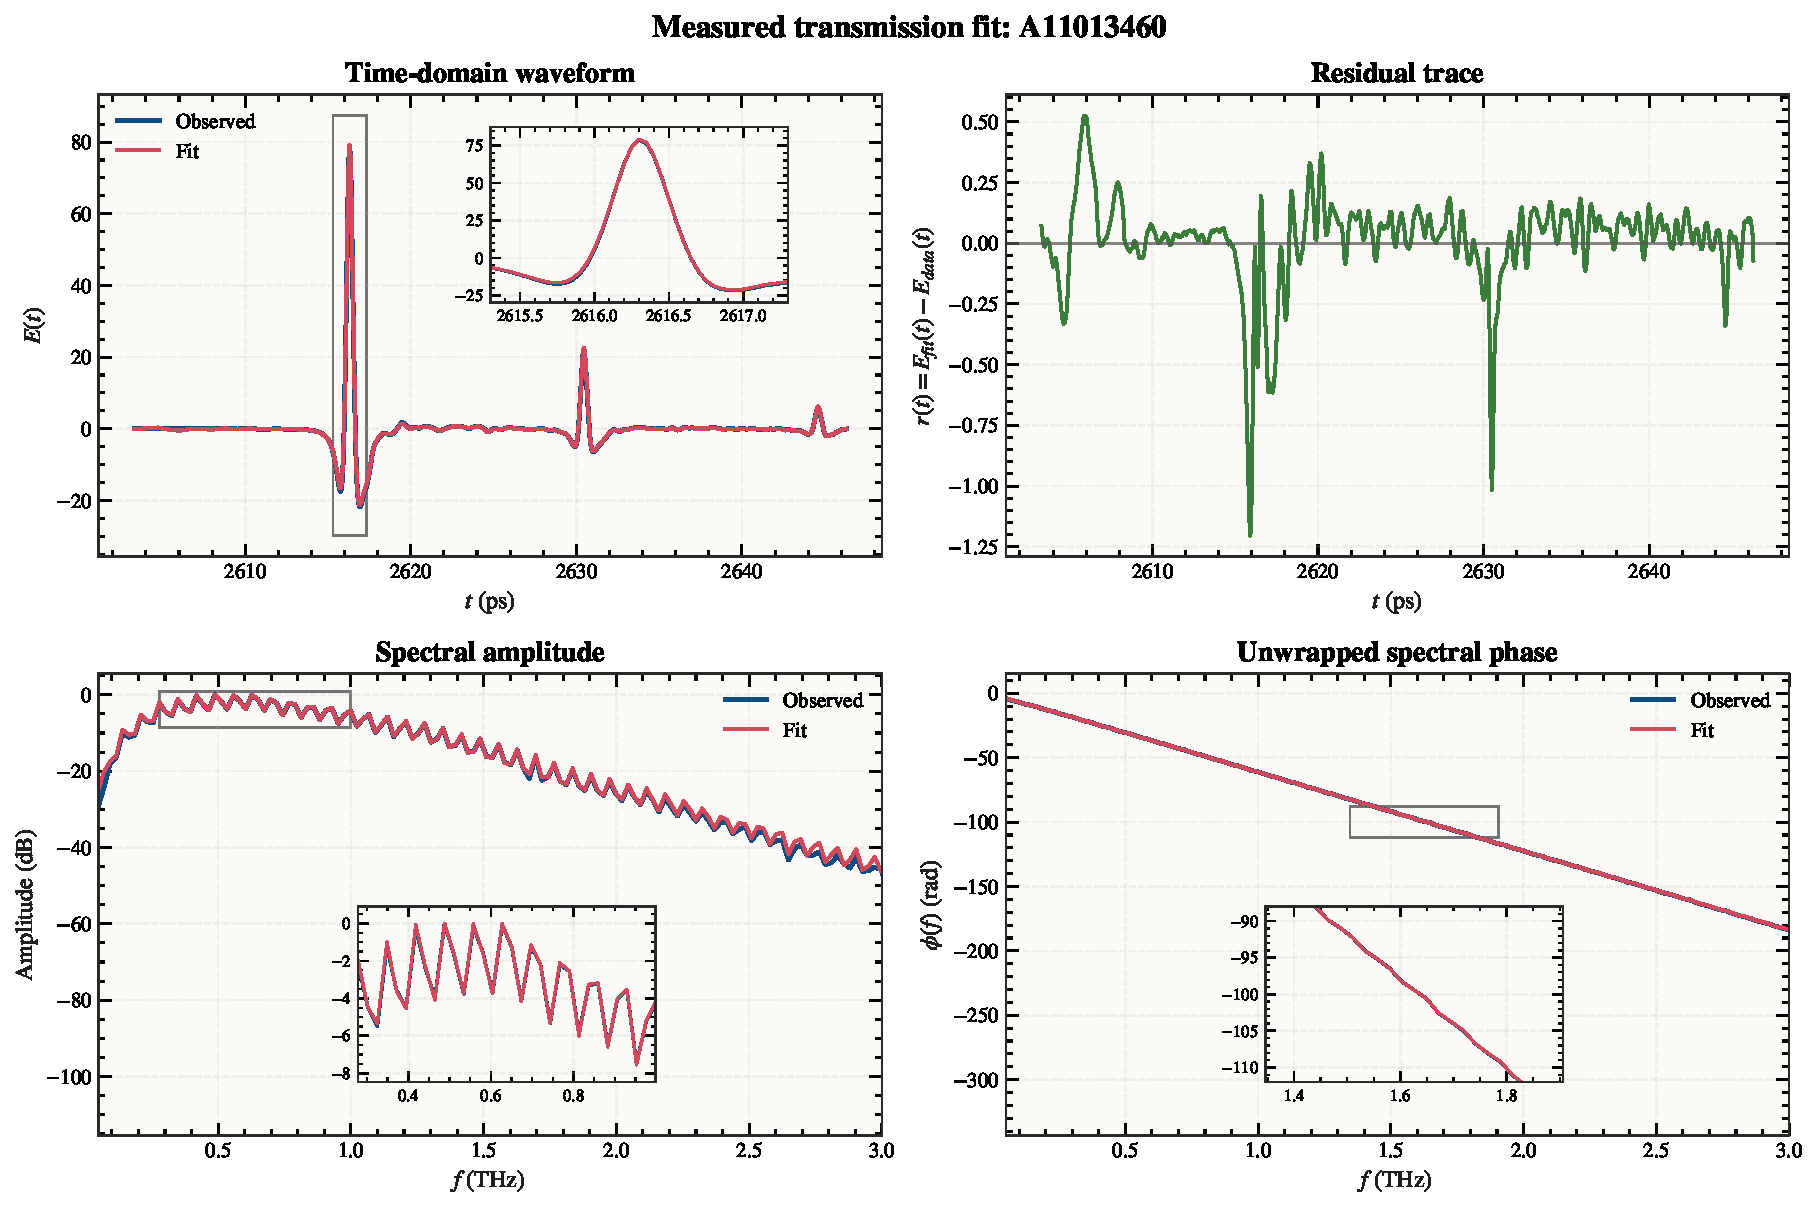
\includegraphics[width=\linewidth]{lecture_build/notebook_measured_transmission/figures/measured_transmission_overview_section.pdf}
\caption{Measured transmission fit for A11013460. The waveform overlay and residual show that the dominant transmitted pulse is reproduced closely, and the spectral amplitude and phase panels remain consistent over the saved usable band. The residual is small but not zero, so the remaining disagreement should still be read as a combination of noise, preprocessing choices, and one-layer-model incompleteness.}
\label{fig:measured-transmission-overview-results}
\end{figure}

\begin{figure}[htbp]
\centering
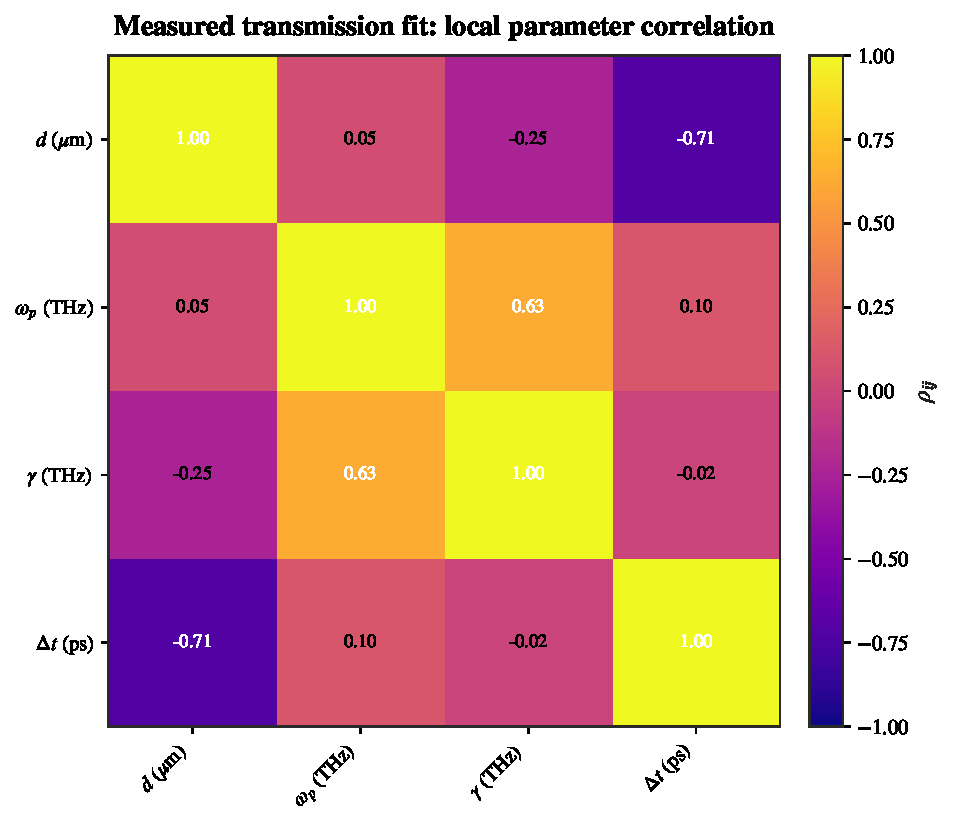
\includegraphics[width=0.62\linewidth]{lecture_build/notebook_measured_transmission/figures/measured_transmission_correlation_section.pdf}
\caption{Local parameter-correlation matrix for the measured transmission fit. The main features are the expected thickness-delay trade-off and the positive plasma-frequency--damping correlation. The matrix shows real coupling, but it does not collapse into a nearly singular nuisance block, which is why this transmission fit is the stronger measured example.}
\label{fig:measured-transmission-correlation-results}
\end{figure}

The transmission fit is the more trustworthy measured example in this lecture set. Its residual is visibly and numerically lower than the reflection residual, and the strongest local couplings have clear physical interpretations rather than looking like arbitrary nuisance absorption. Thickness and delay both shift the waveform in time, so their trade-off is expected. Plasma frequency and damping rate both shape the low-frequency conductivity and spectral roll-off, so their positive correlation is also physically natural. This still does not make the result a complete material characterization: the model is a single effective Drude slab and the residual does not vanish. What it does show is that the measured transmission trace contains enough timing, phase, and amplitude information to constrain a conductivity-oriented wafer fit in a way that remains physically readable.

\subsection{Measured Reflection Fit}

The measured reflection example uses the A11013460 sample trace with an explicit Au-mirror reference pair. The same general fitting logic is used, but the reflection observable is much more sensitive to the reference standard, front-surface phase convention, angle, polarization, scale, and offset. Over the saved \SIrange{1023.7}{1063.8}{ps} crop window, the recovered wafer thickness is \SI{659.08}{\micro\meter}. The Drude parameters are \(\omega_p=\SI{0.1174}{THz}\), \(\gamma=\SI{0.2518}{THz}\), equivalently \(\tau=\SI{0.6321}{ps}\) and \(\sigma=\SI{3.043}{S/m}\). With \(m^\ast=0.26m_e\), the derived carrier density is \(N\approx \SI{4.44e13}{cm^{-3}}\). The weighted waveform objective is \(2.00\times10^{-3}\), the relative \(L_2\) residual is \(6.73\%\), the residual RMS is \(0.1812\), and the estimated fit SNR is \SI{23.44}{dB}. The fitted nuisance parameters include an effective angle of \SI{21.58}{\degree}, a trace scale of \(-0.962\), and a trace offset of \(0.104\).

\begin{figure}[htbp]
\centering
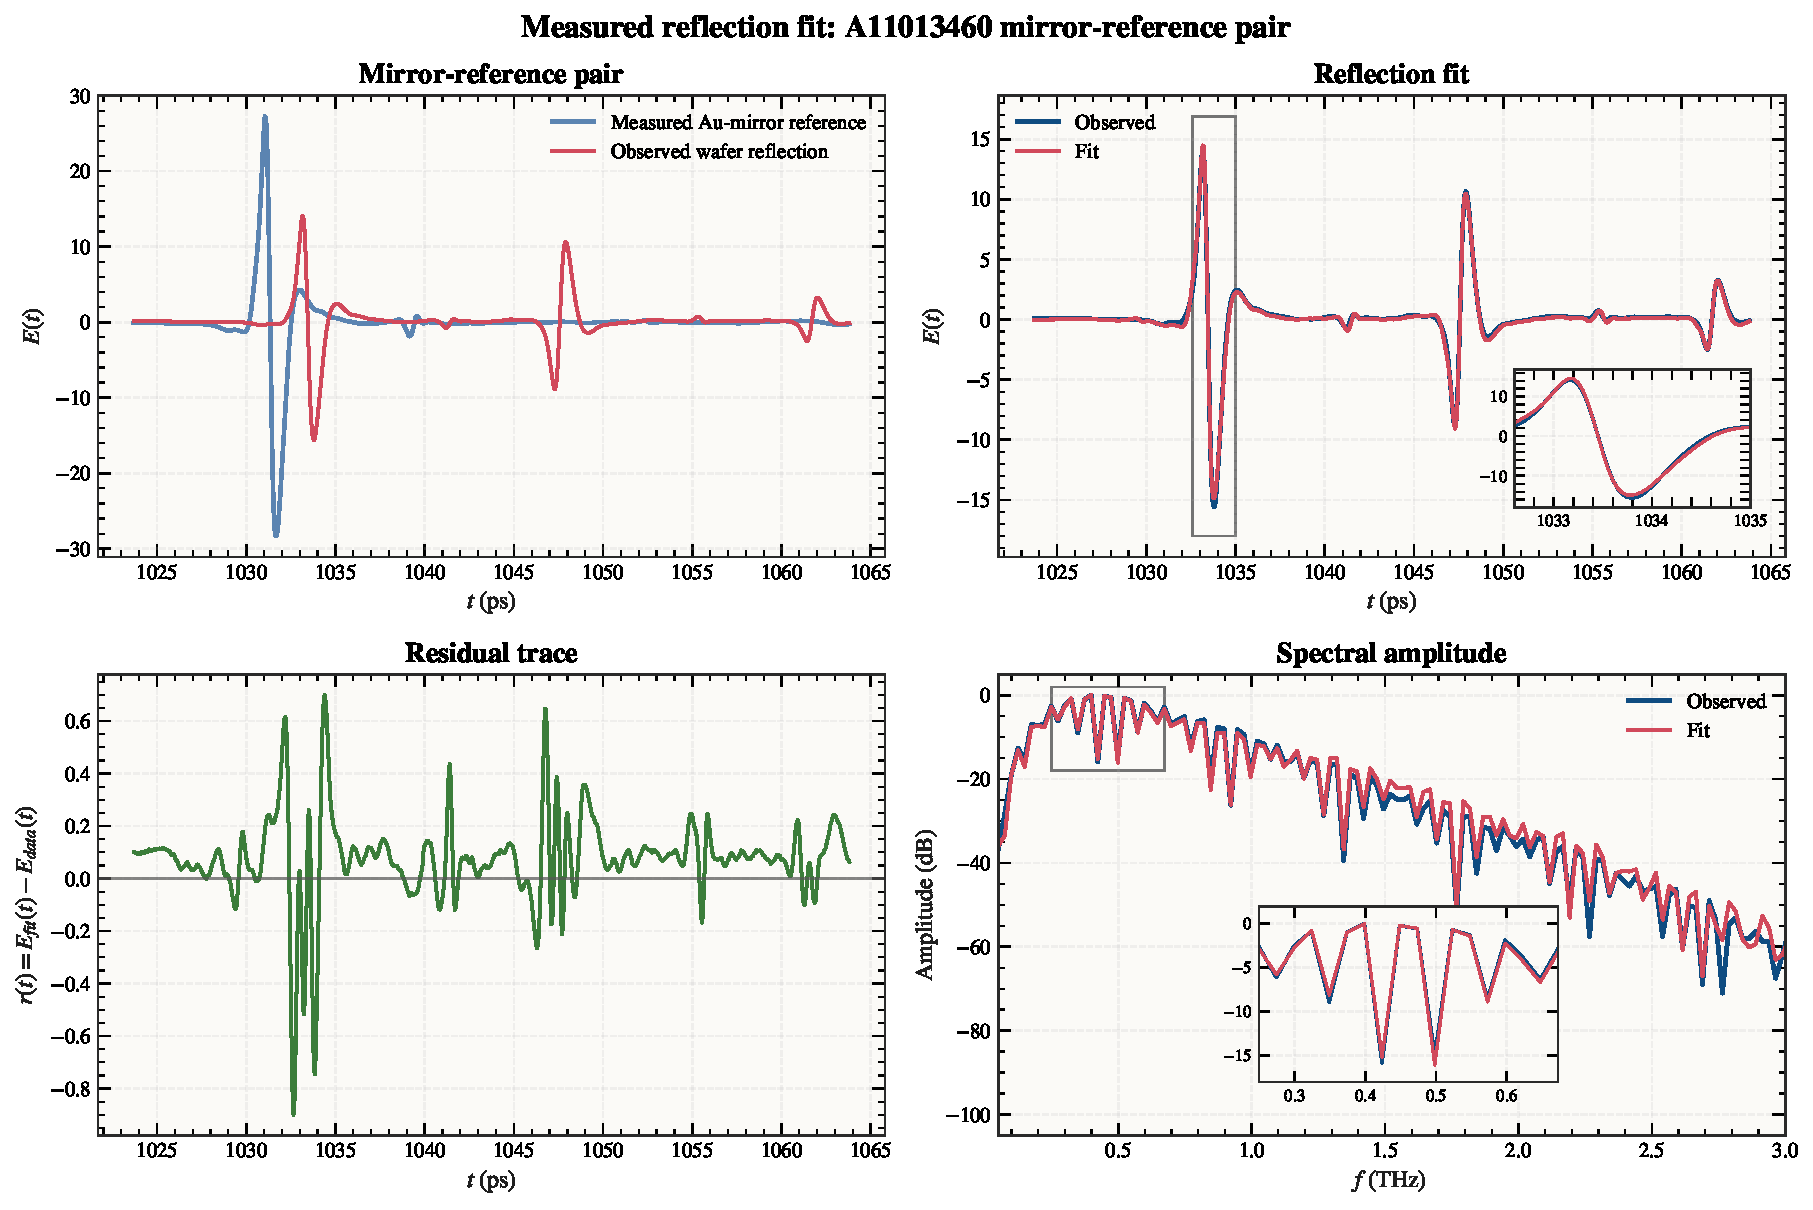
\includegraphics[width=\linewidth]{lecture_build/notebook_measured_reflection/figures/measured_reflection_overview_section.pdf}
\caption{Measured reflection fit for A11013460 using the mirror-reference pair. The fit still captures the main reflected waveform, but the normalized residual is larger than in transmission. In reflection, small errors in the standard, angle, timing, or front-surface response can be traded against fitted material parameters more easily than in the transmission example.}
\label{fig:measured-reflection-overview-results}
\end{figure}

\begin{figure}[htbp]
\centering
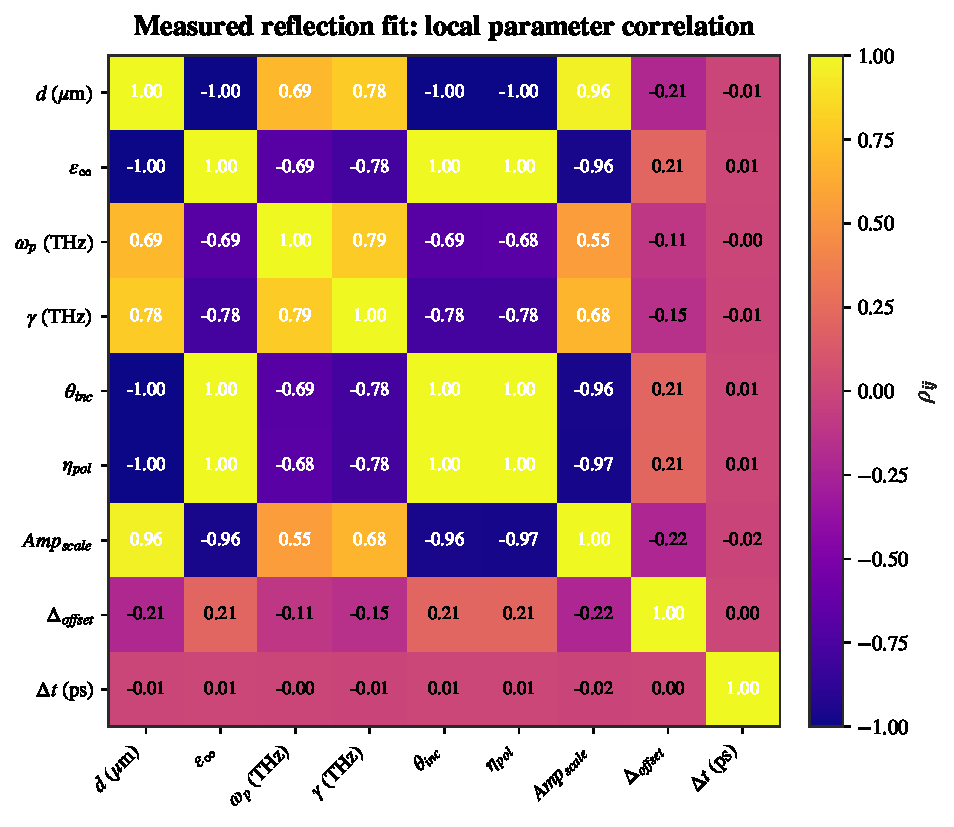
\includegraphics[width=0.62\linewidth]{lecture_build/notebook_measured_reflection/figures/measured_reflection_correlation_section.pdf}
\caption{Local parameter-correlation matrix for the measured reflection fit. The near-perfect couplings between wafer thickness, background permittivity, fitted angle, polarization mix, and trace scale are the main warning sign. This is exactly the kind of local structure that makes a numerical Jacobian-based uncertainty unstable and the resulting material interpretation tentative.}
\label{fig:measured-reflection-correlation-results}
\end{figure}

The reflection fit is therefore a useful demonstration but a more tentative material extraction. The residual is visibly and numerically larger than in transmission, and the local correlation matrix is almost singular in the block that mixes physical wafer properties with measurement nuisance parameters. This does not mean the reflection trace contains no material information. It means that, under the present standard and fit parameterization, the available reflection data do not cleanly separate material response from geometry and normalization. In practice, the fitted \(\tau\), \(\sigma\), and \(N\) should therefore be treated as provisional point estimates rather than robust metrology numbers. A more constrained angle, a better characterized reference standard, a joint transmission-reflection fit, or fewer free nuisance parameters would be needed before giving the reflection fit the same practical weight as the transmission result.

\section{Study Results}

All study results discussed here are generated from the saved notebook outputs. The full maps use a \SI{110}{dB} synthetic dynamic range and the tighter local optimizer settings used in the final notebook run. The plotted study quantities are parameter-recovery errors and related derived errors, not merely waveform residuals. This distinction is essential: a case can fit the synthetic waveform well and still return the wrong conductivity or carrier density if the inverse problem is non-unique. The saved study summaries do not export an explicit spectral fit band, so the notes report the stored time-domain sample counts and map definitions rather than inventing a bandwidth line that is not present in the saved artifacts.

\subsection{One-Layer Drude Study}

The one-layer study uses the optical stack shown in Table~\ref{tab:one-layer-stack-results}. The sample is a single Drude slab between air on both sides, with \(\varepsilon_\infty=11.7\). The low-conductivity cases use \(d=\SI{525}{\micro\meter}\) and \(\sigma\in[\SI{0.01}{S/m},\SI{1}{S/m}]\). The high-conductivity cases use \(d=\SI{725}{\micro\meter}\) and \(\sigma\in[\SI{100}{S/m},\SI{1000}{S/m}]\). In every one-layer map the swept plane is \((\tau,\sigma)\), the synthetic truth and the fit both include up to eight internal reflections, and the reference standard is the identity standard.

\begin{table}[htbp]
\centering
\begin{threeparttable}
\caption{One-layer Drude study construction. The stack is intentionally simple so that the comparison stays focused on geometry and conductivity regime rather than on multilayer complexity.}
\label{tab:one-layer-stack-results}
\small
\begin{tabularx}{\linewidth}{@{}p{3.2cm}p{4.3cm}Y@{}}
\toprule
Element & Setting & Role \\
\midrule
Incident and exit media & air / air & external media for transmission or reflection \\
Fitted layer & Drude slab, \(\varepsilon_\infty=11.7\) & unknown \(\tau\), \(\sigma\), and bounded thickness \\
Low-conductivity geometry & \(d=\SI{525}{\micro\meter}\) & \(\sigma=\SIrange{0.01}{1}{S/m}\), \(\tau=\SIrange{0.1}{1.0}{ps}\) \\
High-conductivity geometry & \(d=\SI{725}{\micro\meter}\) & \(\sigma=\SIrange{100}{1000}{S/m}\), \(\tau=\SIrange{0.1}{1.0}{ps}\) \\
Noise and echoes & \SI{110}{dB}, 8 internal reflections & same forward model for truth and fit \\
\bottomrule
\end{tabularx}
\end{threeparttable}
\end{table}

\begin{figure}[htbp]
\centering
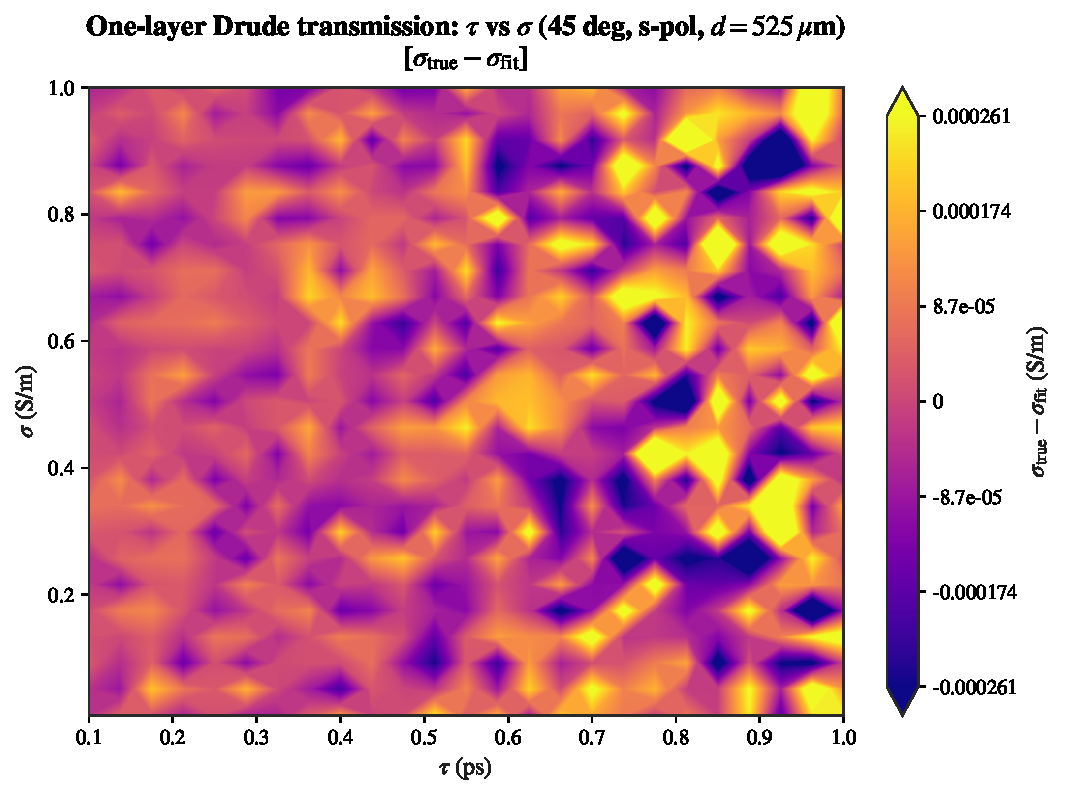
\includegraphics[width=\linewidth]{lecture_build/notebook_section_runs/full_one_layer_tx_tau_sigma_low_s_45deg/data/one_layer/one_layer_tx_tau_sigma_low_s_45deg/one_layer_tx_tau_sigma_low_s_45deg__section_sigma_linear.pdf}
\caption{Representative low-conductivity one-layer transmission map shown in \(\sigma\)-error form. The important visual feature is that the absolute conductivity error remains uniformly small over the plane, which is why this case is a strong metrology configuration rather than merely a good waveform fit.}
\label{fig:one-layer-low-transmission-results}
\end{figure}

\begin{figure}[htbp]
\centering
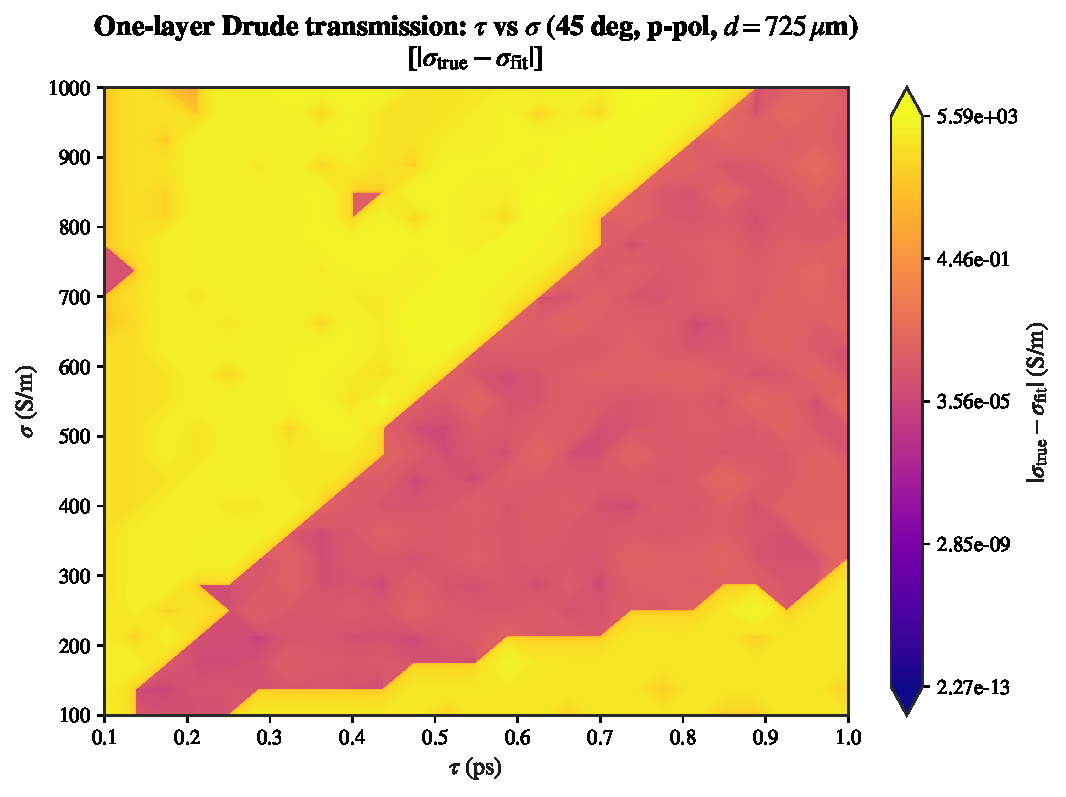
\includegraphics[width=\linewidth]{lecture_build/notebook_section_runs/full_one_layer_tx_tau_sigma_high_p_45deg/data/one_layer/one_layer_tx_tau_sigma_high_p_45deg/one_layer_tx_tau_sigma_high_p_45deg__section_sigma_log.pdf}
\caption{High-conductivity one-layer transmission at \SI{45}{\degree}, p polarization, displayed on the saved logarithmic conductivity-error scale. The point to notice is the broad non-uniform error structure: large parts of the plane admit strongly biased \(\sigma\) recovery even though the optimizer is free to move away from its initial value.}
\label{fig:one-layer-high-transmission-results}
\end{figure}

\begin{figure}[htbp]
\centering
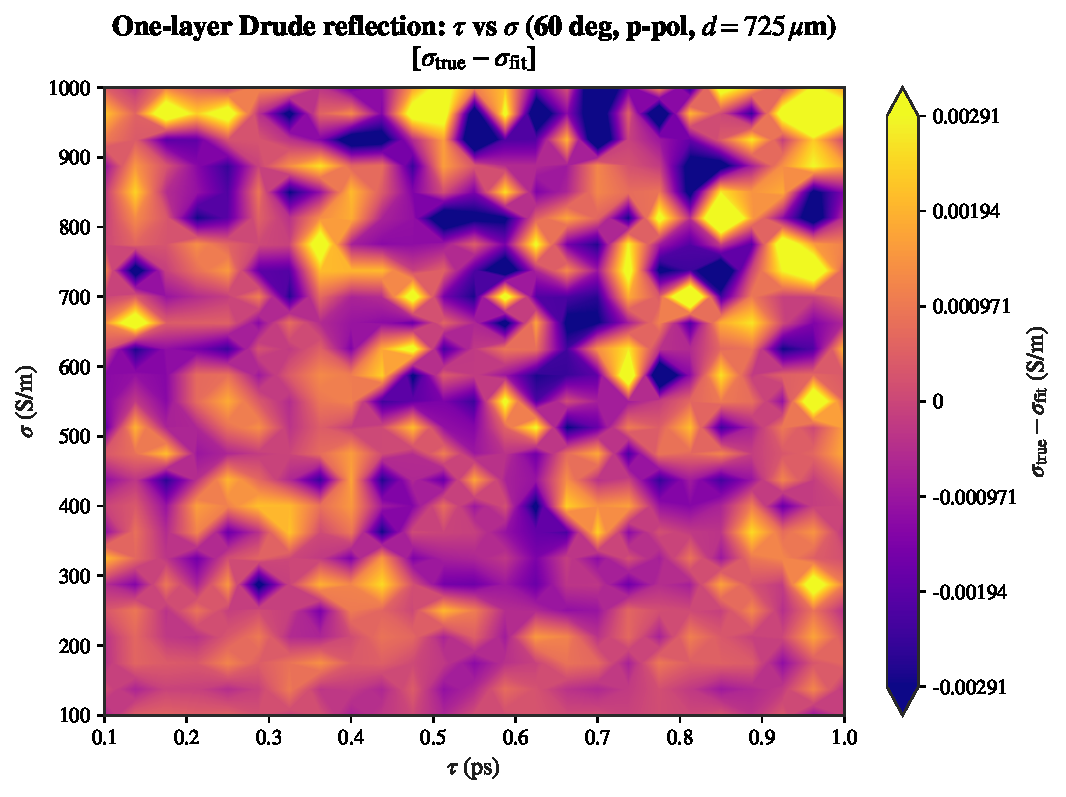
\includegraphics[width=\linewidth]{lecture_build/notebook_section_runs/full_one_layer_refl_tau_sigma_high_p_60deg/data/one_layer/one_layer_refl_tau_sigma_high_p_60deg/one_layer_refl_tau_sigma_high_p_60deg__section_sigma_linear.pdf}
\caption{High-conductivity one-layer reflection at \SI{60}{\degree}, p polarization, again shown directly in \(\sigma\)-error form. Here the map stays close to zero over the entire plane, which is the practical signature of strong high-conductivity recovery in this oblique p-polarized reflection geometry.}
\label{fig:one-layer-high-reflection-results}
\end{figure}

\begin{figure}[htbp]
\centering
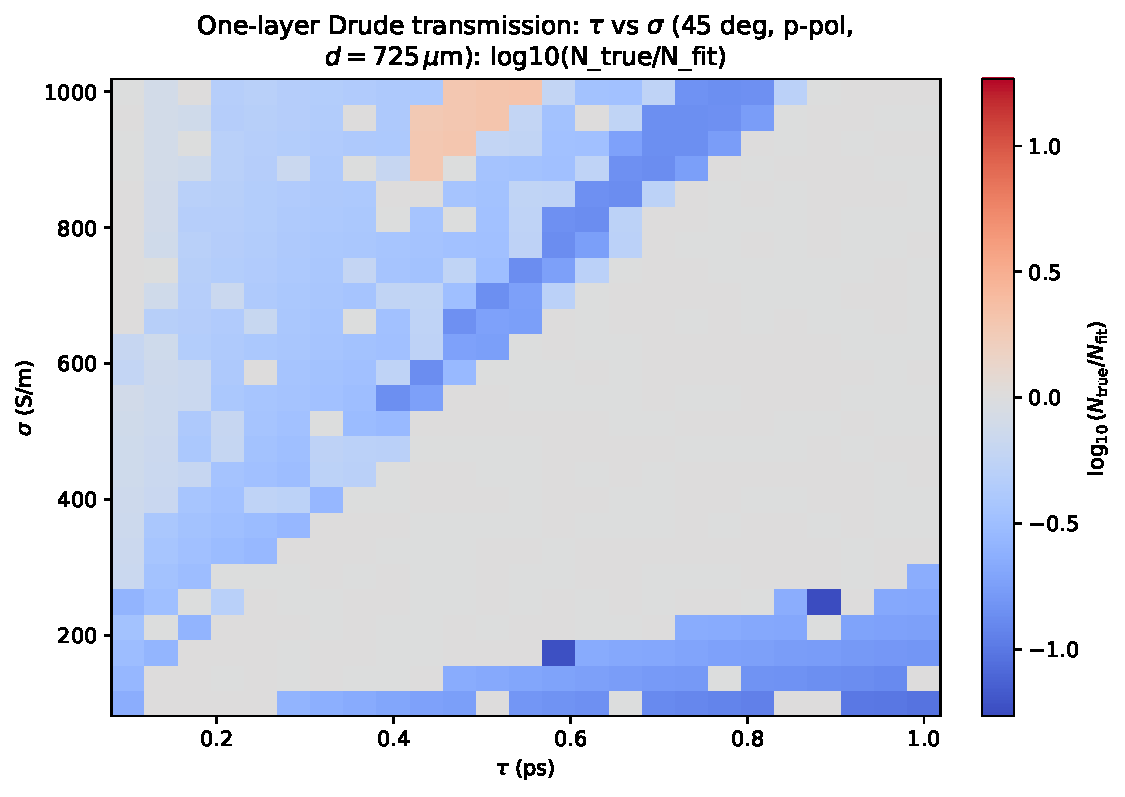
\includegraphics[width=0.48\linewidth]{lecture_build/notebook_section_runs/savecopy6_carrier_density_maps/one_layer_tx_tau_sigma_high_p_45deg__n_signed_log_ratio.pdf}
\hfill
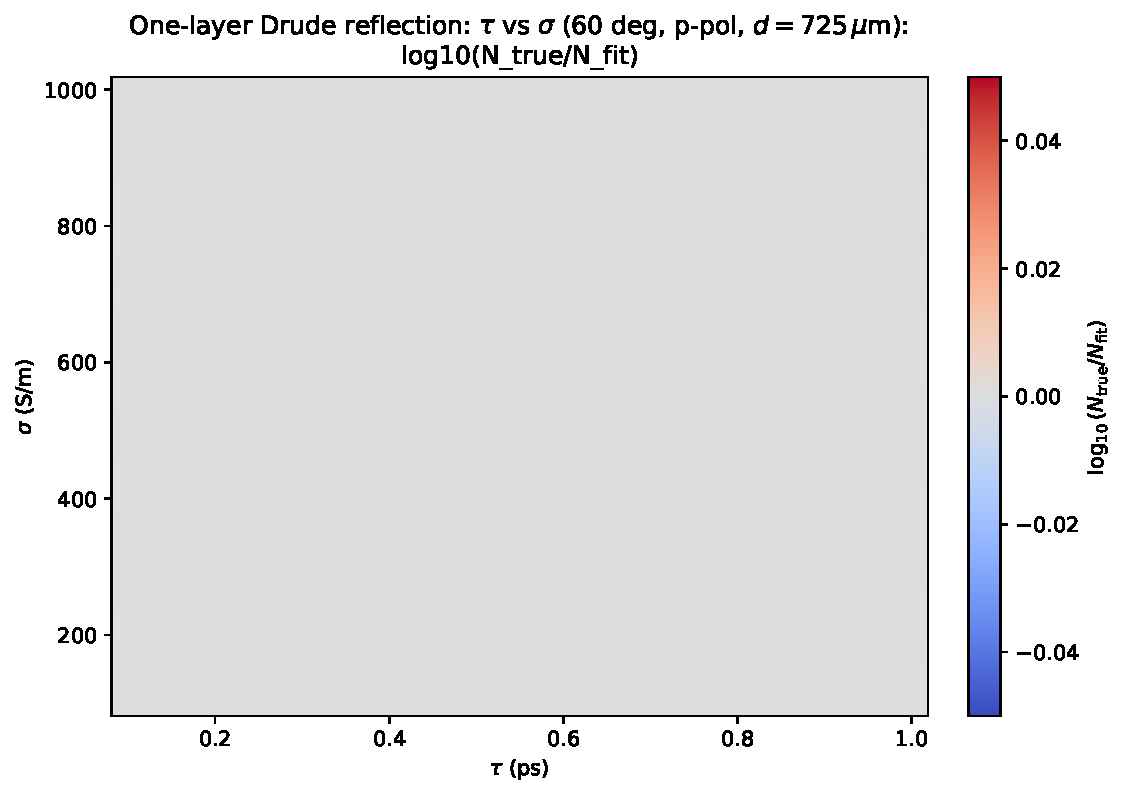
\includegraphics[width=0.48\linewidth]{lecture_build/notebook_section_runs/savecopy6_carrier_density_maps/one_layer_refl_tau_sigma_high_p_60deg__n_signed_log_ratio.pdf}
\caption{Derived carrier-density recovery for two high-conductivity one-layer cases. The left panel shows a real directional bias in \(\log_{10}(N_{\mathrm{true}}/N_{\mathrm{fit}})\) for the non-unique transmission case. The right panel is nearly flat because the carrier-density error is genuinely tiny across the plane, which should be read as near-perfect recovery rather than as a plotting failure. Positive values mean the fit underestimates \(N\), while negative values mean it overestimates \(N\).}
\label{fig:one-layer-carrier-density-contrast-results}
\end{figure}

\begin{table}[htbp]
\centering
\begin{threeparttable}
\caption{One-layer study summary from the saved full-resolution maps, rewritten around conductivity and derived carrier-density recovery.}
\label{tab:one-layer-study-summary-results}
\scriptsize
\begin{tabularx}{\linewidth}{@{}p{2.0cm}p{1.1cm}p{1.4cm}S[table-format=1.2e1]S[table-format=1.2e1]S[table-format=1.2]Y@{}}
\toprule
Regime & Mode & Setup & {$p90\,|\Delta\sigma|$} & {$p90\,|\log_{10}(N_t/N_f)|$} & {Stuck} & Reading \\
\midrule
low, 525 \(\mu\)m & trans. & \(0^\circ\), s & 3.33e-4 & 4.33e-4 & 0.00 & excellent \\
low, 525 \(\mu\)m & trans. & \(45^\circ\), s & 2.61e-4 & 3.80e-4 & 0.00 & excellent \\
high, 725 \(\mu\)m & trans. & \(0^\circ\), s & 2.74e3 & 7.32e-1 & 0.00 & non-unique \\
high, 725 \(\mu\)m & trans. & \(45^\circ\), p & 2.76e3 & 7.33e-1 & 0.00 & non-unique \\
low, 525 \(\mu\)m & refl. & \(45^\circ\), s & 3.08e-4 & 3.92e-4 & 0.00 & excellent \\
low, 525 \(\mu\)m & refl. & \(60^\circ\), s & 3.52e-4 & 3.72e-4 & 0.00 & excellent \\
high, 725 \(\mu\)m & refl. & \(45^\circ\), p & 5.20e-3 & 2.99e-6 & 0.00 & excellent refl. \\
high, 725 \(\mu\)m & refl. & \(60^\circ\), p & 2.91e-3 & 1.98e-6 & 0.00 & excellent refl. \\
\bottomrule
\end{tabularx}
\begin{tablenotes}[flushleft]
\footnotesize
\item \(p90\) denotes the 90th percentile over all map points in the saved full-resolution study.
\item Stuck fraction is the fraction of map points flagged by the notebook's stuck-to-initial diagnostic.
\item Setup lists angle and polarization; conductivity units are S/m.
\item The \(N\) metric is \( |\log_{10}(N_{\mathrm{true}}/N_{\mathrm{fit}})| \) with \( \mstar = 0.26m_e \).
\item Each saved map contains 625 truth points (\(25\times25\)), each synthetic fitted trace contains 1024 time-domain samples, and the saved final study run uses \SI{110}{dB} synthetic dynamic range.
\end{tablenotes}
\end{threeparttable}
\end{table}

The one-layer maps make a clean physical point. In the low-conductivity regime, both transmission and reflection recover \(\sigma\) and the derived \(N\) extremely well. The measured waveform remains sensitive to the small Drude perturbation, and the inverse problem is locally and globally stable at the imposed noise level. In the high-conductivity regime the behavior separates by measurement mode. Reflection, especially the p-polarized \SI{60}{\degree} case, becomes highly sensitive to the conductive surface response and recovers \(\sigma\) almost exactly. Transmission, however, becomes globally ambiguous. The synthetic transmitted waveform can be reproduced with conductivities far above the truth in parts of the map, so the recovery map correctly marks this as a poor metrology configuration even though the optimizer is not stuck at its initial value.

\subsection{Two-Drude / Advanced Epi Study}

The advanced study uses a wafer-style stack with a two-Drude epi layer, a thin oxide, and a finite substrate. The model stack is air / epi / oxide / substrate / air. The epi has \(\varepsilon_\infty=11.7\) and two Drude channels; the oxide has \(d_{\mathrm{ox}}=\SI{10}{\micro\meter}\), \(n=1.95\), and \(k=0.005\); the substrate has \(n=3.42\) and \(k=0.005\). Transmission uses the identity reference standard. Reflection uses a stack reference standard consisting of the oxide and substrate without the conductive epi layer.

\begin{table}[htbp]
\centering
\begin{threeparttable}
\caption{Advanced epi study configurations used in the final notebook output. Each \((\tau_i,\sigma_i)\) map sweeps one Drude channel while the other channel is fixed at its nominal pair value.}
\label{tab:advanced-stack-results}
\small
\begin{tabularx}{\linewidth}{@{}p{2.8cm}p{4.8cm}p{1.9cm}p{1.9cm}Y@{}}
\toprule
Geometry & Stack thicknesses & Transmission cases & Reflection cases & Reference \\
\midrule
525-\(\mu\)m substrate & \(d_{\mathrm{epi}}=\SI{50}{\micro\meter}\), \(d_{\mathrm{ox}}=\SI{10}{\micro\meter}\), \(d_{\mathrm{sub}}=\SI{525}{\micro\meter}\) & \SI{0}{\degree}, s & \SI{45}{\degree}, s & oxide+substrate for reflection \\
725-\(\mu\)m substrate & \(d_{\mathrm{epi}}=\SI{70}{\micro\meter}\), \(d_{\mathrm{ox}}=\SI{10}{\micro\meter}\), \(d_{\mathrm{sub}}=\SI{725}{\micro\meter}\) & \SI{45}{\degree}, s & \SI{60}{\degree}, s & oxide+substrate for reflection \\
\bottomrule
\end{tabularx}
\end{threeparttable}
\end{table}

\begin{figure}[htbp]
\centering
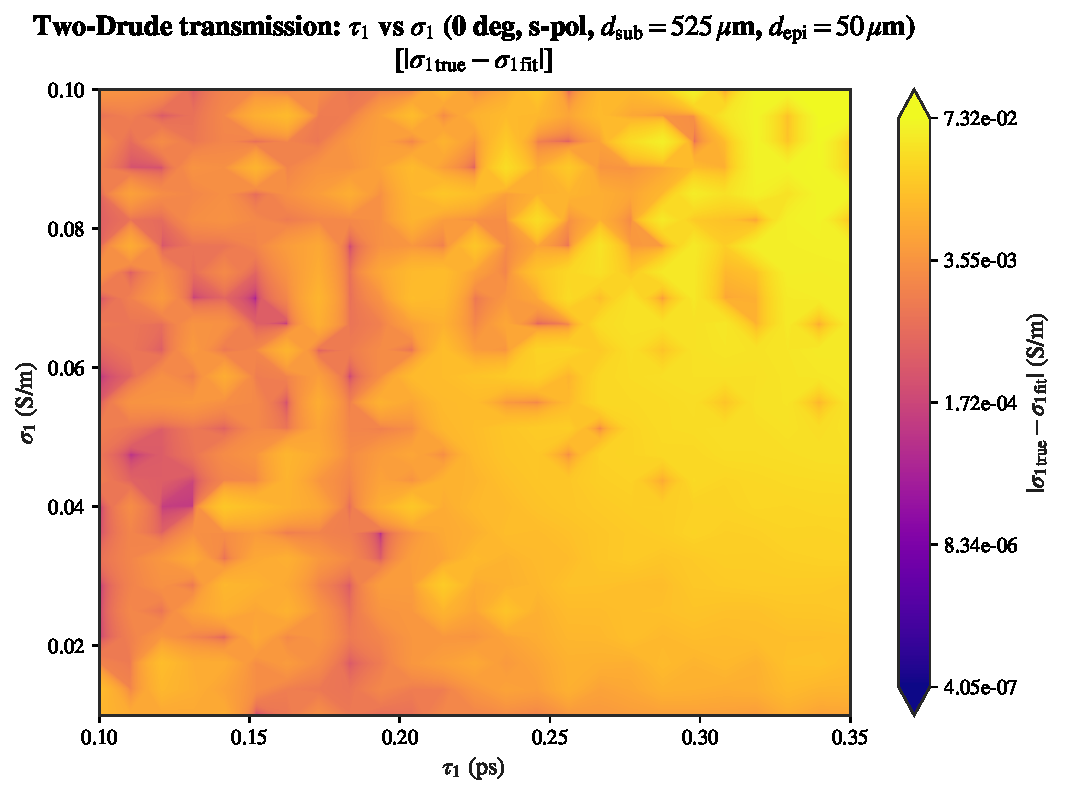
\includegraphics[width=\linewidth]{lecture_build/notebook_section_runs/full_advanced_tx_tau1_sigma1_0deg_s_525um/data/advanced/advanced_tx_tau1_sigma1_0deg_s_525um/advanced_tx_tau1_sigma1_0deg_s_525um__section_sigma_log.pdf}
\caption{Two-Drude transmission for channel 1 in the \SI{525}{\micro\meter} substrate geometry, displayed in the saved logarithmic conductivity-error view. The useful reading is that conductivity recovery is only moderate here: the structure is better than a stuck map, but it is not uniformly close to zero over the plane.}
\label{fig:advanced-tx-channel1-moderate-results}
\end{figure}

\begin{figure}[htbp]
\centering
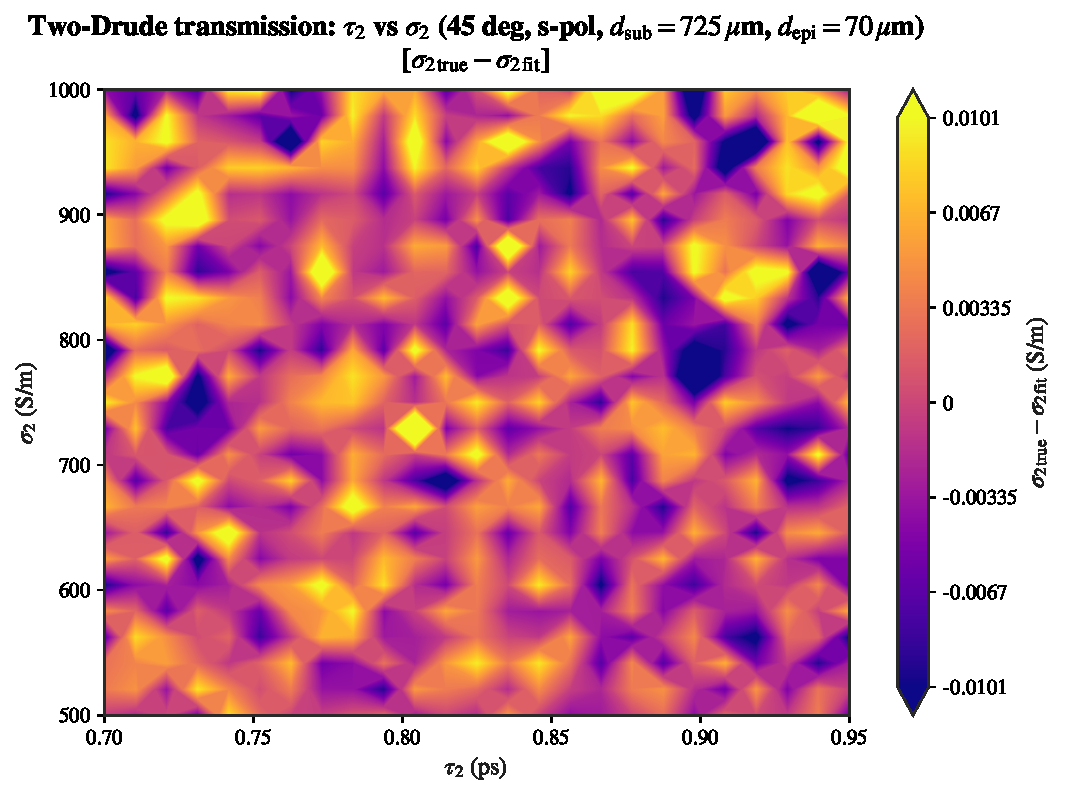
\includegraphics[width=\linewidth]{lecture_build/notebook_section_runs/full_advanced_tx_tau2_sigma2_45deg_s_725um/data/advanced/advanced_tx_tau2_sigma2_45deg_s_725um/advanced_tx_tau2_sigma2_45deg_s_725um__section_sigma_linear.pdf}
\caption{Two-Drude transmission for channel 2 in the \SI{725}{\micro\meter} substrate geometry, now shown directly in absolute conductivity error. The map stays close to zero across the plane, which is why this is one of the strongest advanced transmission cases for conductivity and derived carrier density.}
\label{fig:advanced-tx-channel2-excellent-results}
\end{figure}

\begin{figure}[htbp]
\centering
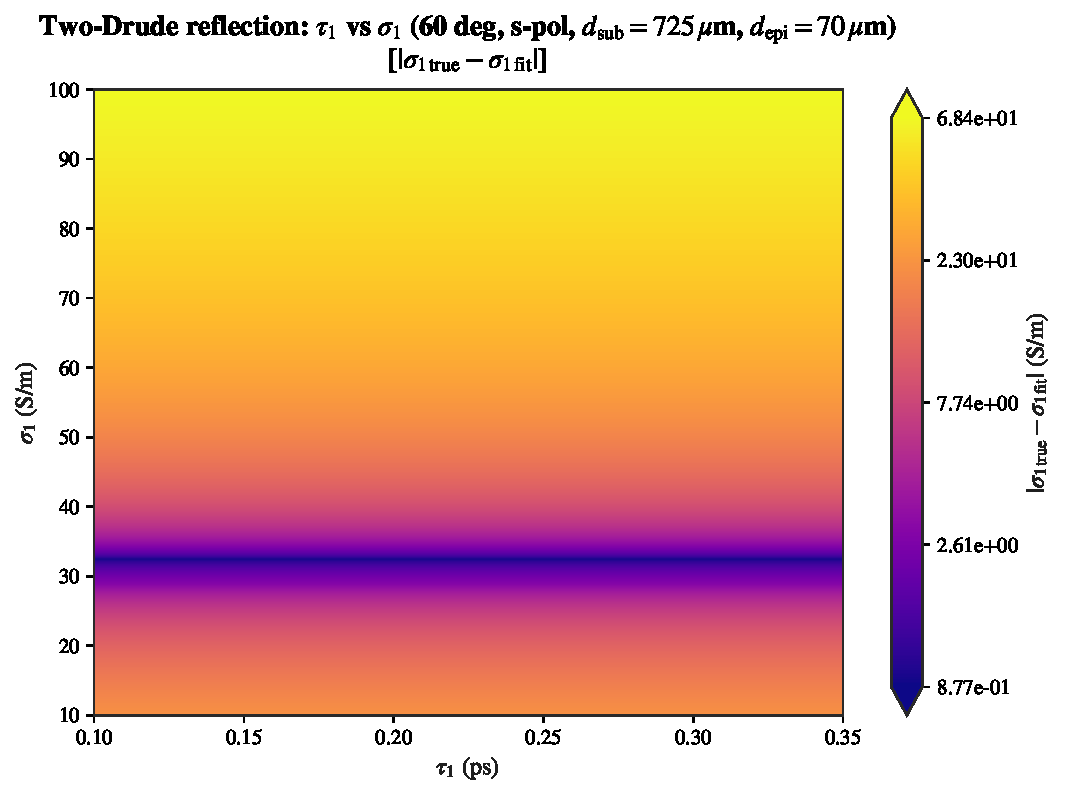
\includegraphics[width=\linewidth]{lecture_build/notebook_section_runs/full_advanced_refl_tau1_sigma1_60deg_s_725um/data/advanced/advanced_refl_tau1_sigma1_60deg_s_725um/advanced_refl_tau1_sigma1_60deg_s_725um__section_sigma_log.pdf}
\caption{Two-Drude reflection for channel 1 in the \SI{725}{\micro\meter} substrate geometry, again displayed on the saved logarithmic conductivity-error scale. The main message is not only that the error is large, but that the map structure is consistent with initial-value-dominated recovery failure rather than a cleanly recoverable channel.}
\label{fig:advanced-reflection-stuck-results}
\end{figure}

\begin{figure}[htbp]
\centering
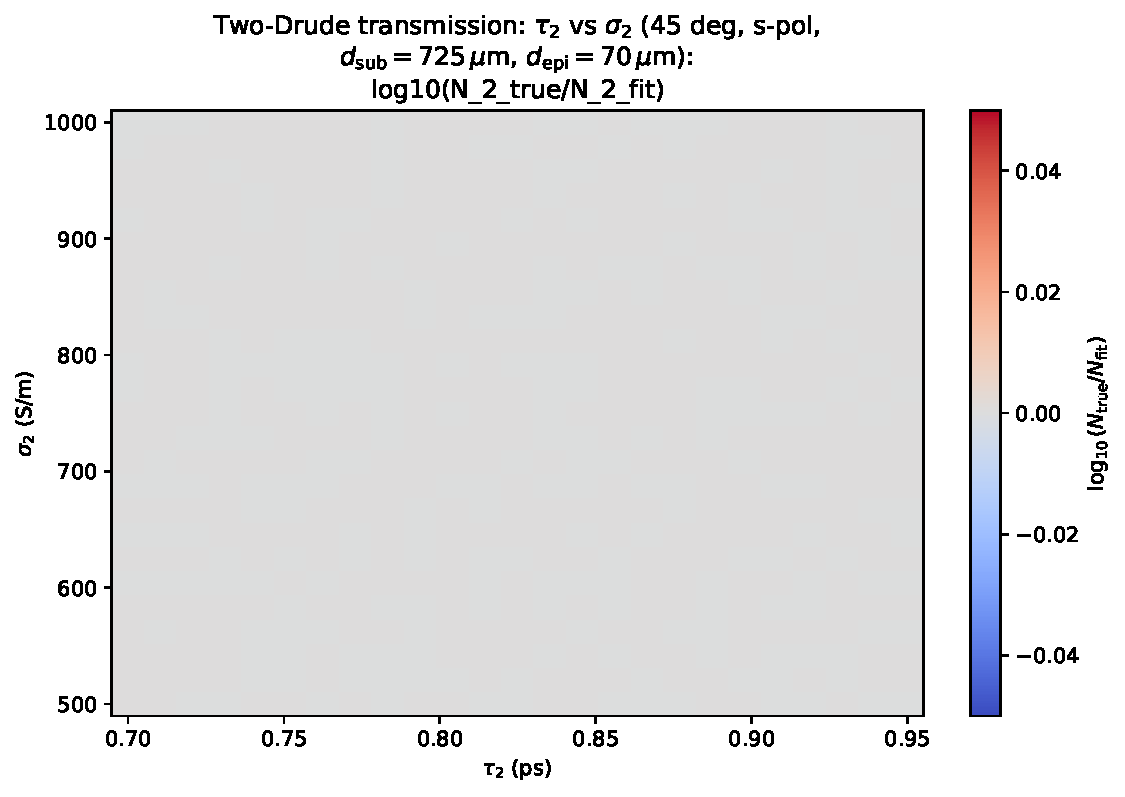
\includegraphics[width=0.48\linewidth]{lecture_build/notebook_section_runs/savecopy6_carrier_density_maps/advanced_tx_tau2_sigma2_45deg_s_725um__n2_signed_log_ratio.pdf}
\hfill
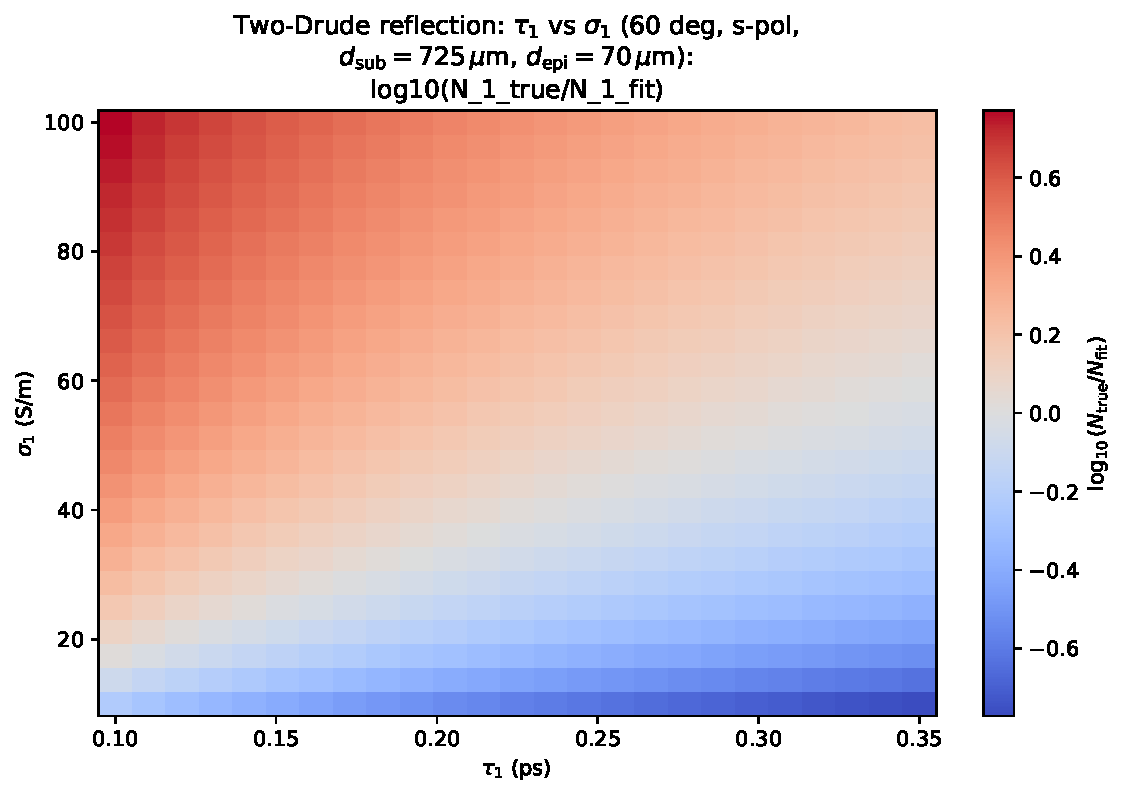
\includegraphics[width=0.48\linewidth]{lecture_build/notebook_section_runs/savecopy6_carrier_density_maps/advanced_refl_tau1_sigma1_60deg_s_725um__n1_signed_log_ratio.pdf}
\caption{Derived carrier-density contrast for the advanced epi study. The left panel is almost visually flat because the saved channel-2 transmission recovery is extremely good; the right panel shows a real signed-bias pattern for the reflection failure case. This is a useful reminder that a bland carrier-density map can mean either excellent recovery or poor plotting choice, so the caption must tell the reader which one it is.}
\label{fig:advanced-carrier-density-contrast-results}
\end{figure}

\begin{table}[htbp]
\centering
\begin{threeparttable}
\caption{Advanced epi study summary from the saved full-resolution maps, with conductivity and derived carrier-density recovery placed ahead of any auxiliary scalar summary.}
\label{tab:advanced-study-summary-results}
\scriptsize
\begin{tabularx}{\linewidth}{@{}p{1.0cm}p{1.1cm}p{2.0cm}S[table-format=2.2e1]S[table-format=1.2e1]S[table-format=1.2]Y@{}}
\toprule
Ch. & Mode & Setup & {$p90\,|\Delta\sigma|$} & {$p90\,|\log_{10}(N_t/N_f)|$} & {Stuck} & Reading \\
\midrule
1 & trans. & 525/50, \(0^\circ\), s & 3.57e-2 & 2.54e-1 & 0.00 & moderate \\
2 & trans. & 525/50, \(0^\circ\), s & 2.88e-3 & 3.55e-3 & 0.00 & excellent \\
1 & trans. & 725/70, \(45^\circ\), s & 5.19e-2 & 3.84e-4 & 0.00 & good \\
2 & trans. & 725/70, \(45^\circ\), s & 1.01e-2 & 1.84e-5 & 0.00 & excellent \\
1 & refl. & 525/50, \(45^\circ\), s & 6.09e-2 & 5.50e-1 & 1.00 & stuck \\
2 & refl. & 525/50, \(45^\circ\), s & 1.16e-1 & 9.15e-2 & 0.96 & mostly stuck \\
1 & refl. & 725/70, \(60^\circ\), s & 6.09e1 & 5.50e-1 & 1.00 & stuck \\
2 & refl. & 725/70, \(60^\circ\), s & 2.51e2 & 1.60e-1 & 1.00 & stuck \\
\bottomrule
\end{tabularx}
\begin{tablenotes}[flushleft]
\footnotesize
\item Setup lists substrate/epi thickness in \(\mu\)m, then angle and polarization; conductivity units are S/m.
\item The definitions of \(p90\), stuck fraction, map size, sample count, and dynamic range are the same as in Table~\ref{tab:one-layer-study-summary-results}.
\end{tablenotes}
\end{threeparttable}
\end{table}

The advanced maps show why two-Drude extraction is a harder wafer-metrology problem than one-Drude extraction. Transmission can work well, but the two channels are not equally recoverable. Channel 2 is recovered very strongly in both transmission geometries, especially for the \SI{725}{\micro\meter} substrate and \SI{70}{\micro\meter} epi case. Channel 1 at normal incidence in the \SI{525}{\micro\meter} geometry is much weaker, with a large p90 carrier-density log error. Reflection is not quantitatively reliable in these advanced cases. The reflection maps do not merely show large noise; they show fitted values returning to the nominal initial channel values over most or all of the map. That is an identifiability failure under the present measurement standard and parameterization.

\section{Discussion and Practical Interpretation}

The strongest lesson from the saved results is that local fit quality and global recoverability are different questions. A single optimized waveform and its local correlation matrix tell us what happens near one optimum. A study map tells us whether the same measurement geometry reliably returns the correct \(\sigma\) and derived \(N\) across an operating region. For metrology, the second question matters more. A waveform can look convincing and still sit inside a globally ambiguous inverse problem.

This distinction is clearest in the one-layer cases. At low conductivity, both transmission and reflection recover \(\sigma\) and the derived carrier density with very small p90 errors. The waveform remains sensitive to the Drude perturbation, and the inverse problem is both locally and globally well behaved. At high conductivity, however, the transmission maps cease to be useful metrology maps even though the optimizer is not merely stuck at its starting point. In those cases the transmitted waveform can still be matched while \(\sigma\) runs far away from the truth, so the problem is global non-uniqueness rather than optimizer paralysis. Reflection behaves differently. In oblique p-polarized high-conductivity reflection the surface response remains strongly conductivity-sensitive, and both \(\sigma\) and the derived \(N\) are recovered extremely well.

The two-Drude maps show that a more realistic epi model comes with a harder identifiability problem. Adding a second conduction channel is physically well motivated for parallel carrier populations or transport paths, but it also creates more ways for spectral weight and scattering time to trade off. The saved transmission results remain genuinely useful, especially for channel 2 and for the \SI{725}{\micro\meter} substrate geometry. Channel 1 in the \SI{525}{\micro\meter} normal-incidence transmission case is only moderate, which means the fit still contains real information but does not support the same level of quantitative confidence. The reflection maps are qualitatively different. Their high stuck fractions and large \(\sigma\) and \(N\) errors show that the current reflection configuration does not separate the two Drude channels robustly.

Carrier density is still the right industrial language only after its assumptions are made explicit. The study outputs convert \((\sigma,\tau)\) to \(N\) using \(\mstar=0.26m_e\), so absolute \(N\) values inherit that effective-mass convention. The signed log-ratio maps remain especially useful because they show relative carrier-density recovery independently of the absolute scale factor. In that sense, \(\sigma\) is the most direct recovered electrical quantity, while \(N\) is the most practical derived output for wafer interpretation once the Drude model and effective mass are accepted.

The measured fits line up with this metrology reading. The measured transmission fit is the stronger real-data example because it pairs a smaller residual with an interpretable local correlation structure. The measured reflection fit is more tentative because physical wafer parameters and nuisance parameters move almost as one block. That does not make reflection useless; it means the present reflection standard and parameterization are not yet strong enough for a high-confidence material extraction. The practical message is therefore not that one geometry is always best. It is that the geometry and reference strategy must be chosen for the parameter that actually matters, and in these notes that parameter is primarily \(\sigma\), with \(N\) following as the derived industrial quantity.

\section{Compact Summary / Industrial Takeaway}

For the present data and study settings, the most robust quantitative paths are low-conductivity one-layer transmission or reflection, high-conductivity one-layer reflection, and two-Drude transmission for the better-conditioned advanced epi channels. The least trustworthy paths are high-conductivity one-layer transmission and two-Drude reflection. This supports a transmission-first strategy for quantitative two-Drude epi metrology, while reflection should be treated as a design target requiring stronger standards, tighter geometry constraints, joint fitting, or fewer free Drude parameters.

\begin{table}[htbp]
\centering
\begin{threeparttable}
\caption{Compact metrology classification of the saved final study set, phrased in terms of conductivity and carrier-density usefulness rather than waveform appearance alone.}
\label{tab:industrial-takeaway-results}
\small
\begin{tabularx}{\linewidth}{@{}p{2.6cm}Y Y@{}}
\toprule
Study family & Sigma / carrier-density takeaway & Practical caution \\
\midrule
One-layer, low conductivity & Excellent \(\sigma\) and \(N\) recovery in both transmission and reflection & \(\tau\)-\(\sigma\) coupling still governs local sensitivity \\
One-layer, high conductivity & Excellent in oblique p-polarized reflection & Transmission becomes globally non-unique even without initial-value sticking \\
Two-Drude transmission & Useful for advanced epi metrology, especially channel 2 and the 725-\(\mu\)m geometry & Channel 1 at 525-\(\mu\)m normal incidence is only moderate \\
Two-Drude reflection & Not ready for quantitative two-channel extraction under the present setup & Maps are dominated by initial-value attraction and channel non-separation \\
Measured transmission & Stronger real-data conductivity-oriented demonstration & Still an effective one-layer description, not a complete wafer model \\
Measured reflection & Useful qualitative reflection example & Material parameters remain tentative because nuisance coupling is nearly singular \\
\bottomrule
\end{tabularx}
\end{threeparttable}
\end{table}

The industrial conclusion is deliberately conservative. THz-TDS time-domain fitting can produce wafer-relevant quantities such as conductivity, scattering time, and carrier density, but confidence maps are needed to decide whether those quantities are actually recoverable for the chosen stack and measurement geometry. In the present results, the most defensible carrier-density conclusions come from the configurations whose \(N_{\mathrm{true}}/N_{\mathrm{fit}}\) maps are flat and close to unity, not from the configurations that merely produce low waveform residuals.

\end{document}
